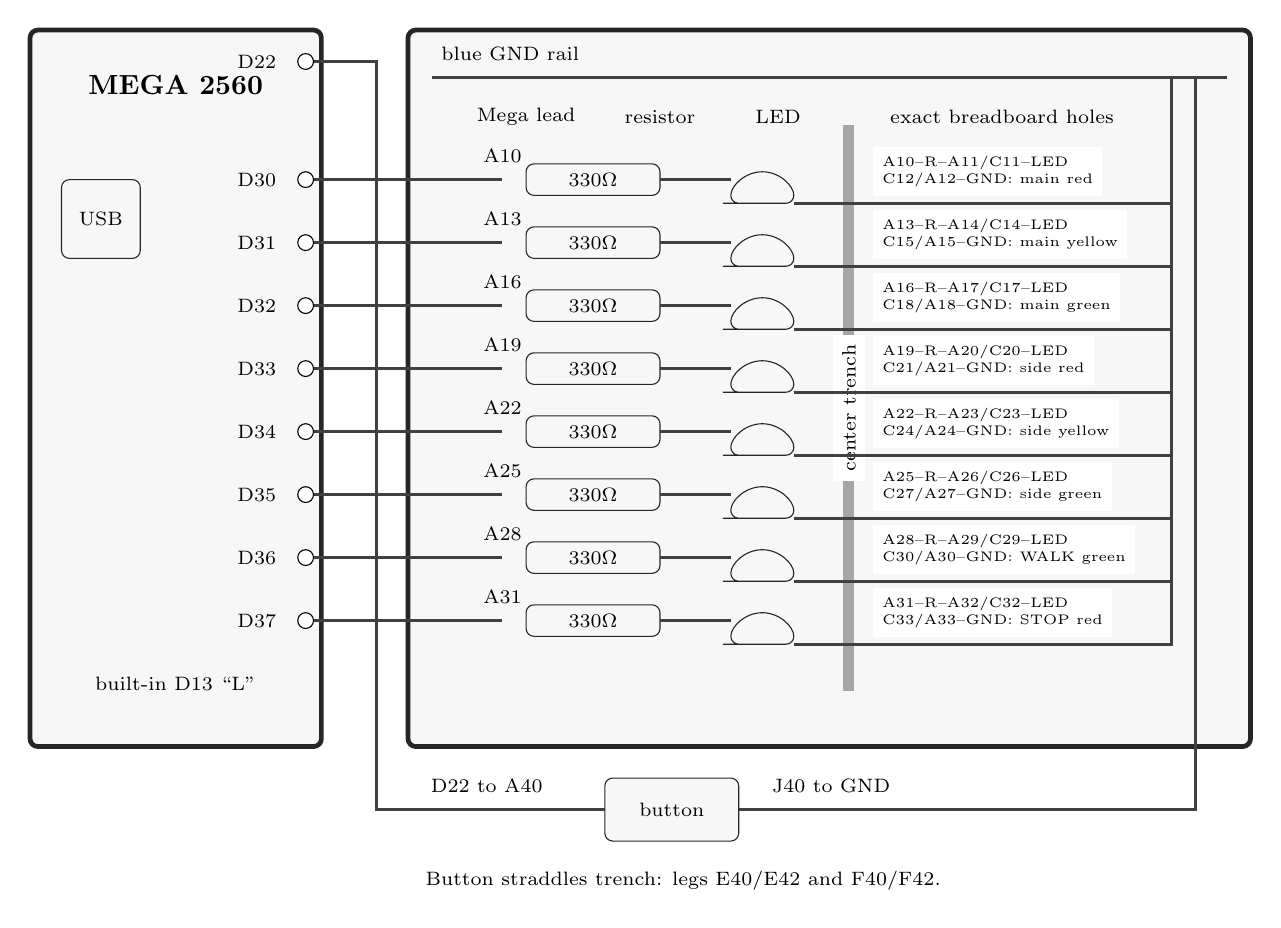
\begin{tikzpicture}[
  x=1mm,y=1mm,
  wire/.style={draw=black!75,line width=0.42mm},
  part/.style={draw=black!85,rounded corners=1mm,fill=black!3},
  note/.style={font=\scriptsize,align=left}]
  \draw[part,line width=0.6mm] (0,0) rectangle (37,91);
  \node[font=\bfseries] at (18.5,84) {MEGA 2560};
  \draw[part] (4,62) rectangle (14,72);
  \node[note] at (9,67) {USB};
  \node[note] at (18.5,8) {built-in D13 ``L''};

  \draw[part,line width=0.6mm] (48,0) rectangle (155,91);
  \draw[wire] (51,85) -- (152,85);
  \node[note,anchor=west] at (51,88) {blue GND rail};
  \draw[black!35,line width=1.4mm] (104,7) -- (104,79);
  \node[note,fill=white,rotate=90] at (104,43) {center trench};
  \node[note] at (63,80) {Mega lead};
  \node[note] at (80,80) {resistor};
  \node[note] at (95,80) {LED};
  \node[note,anchor=west] at (108,80) {exact breadboard holes};

  \foreach \pin/\start/\middle/\finish/\name/\y in {
    30/10/11/12/main red/72,
    31/13/14/15/main yellow/64,
    32/16/17/18/main green/56,
    33/19/20/21/side red/48,
    34/22/23/24/side yellow/40,
    35/25/26/27/side green/32,
    36/28/29/30/WALK green/24,
    37/31/32/33/STOP red/16}
  {
    \draw[fill=white] (35,\y) circle (1);
    \node[note,anchor=east] at (32.5,\y) {D\pin};
    \draw[wire] (36,\y) -- (60,\y);
    \node[note] at (60,\y+3) {A\start};
    \draw[part] (63,\y-2) rectangle (80,\y+2);
    \node[note] at (71.5,\y) {330\(\Omega\)};
    \draw[wire] (80,\y) -- (89,\y);
    \draw[part] (89,\y-3) -- (97,\y-3)
      arc[start angle=0,end angle=180,radius=4mm] -- cycle;
    \draw[wire] (97,\y-3) -- (145,\y-3) -- (145,85);
    \node[font=\tiny,align=left,anchor=west,fill=white] at (107,\y+1)
      {A\start--R--A\middle/C\middle--LED\\
       C\finish/A\finish--GND: \name};
  }

  \draw[fill=white] (35,87) circle (1);
  \node[note,anchor=east] at (32.5,87) {D22};
  \draw[wire] (36,87) -- (44,87) -- (44,-8) -- (73,-8);
  \node[note] at (58,-5) {D22 to A40};
  \draw[part] (73,-12) rectangle (90,-4);
  \node[note] at (81.5,-8) {button};
  \draw[wire] (90,-8) -- (148,-8) -- (148,85);
  \node[note,anchor=west] at (93,-5) {J40 to GND};
  \node[note,anchor=west] at (49,-17)
    {Button straddles trench: legs E40/E42 and F40/F42.};
\end{tikzpicture}
